\chapter{Bitcoin, a peer-to-peer payment network}
\label{chap:bitcoin}

The Bitcoin ecosystem is composed of multiple actors. Users of the network
access information via software on their laptop or mobile phone. These users can
see the amounts present in their addresses. An address is the digest of a public
key, itself being the representation of a private key. An address is owned by a
user if this user has the associated private key in his possession. Users can
transfer funds from some of their addresses to other addresses owned by other
users or themselves. When funds are transferred a transaction is created and
sent to the network. The network is composed of nodes, and these nodes take care
of its proper functioning. Some of these nodes are called miners, they listen to
new transactions and try to include them into the blockchain. This blockchain is
the output, the necessary result, of the Bitcoin protocol and can be compared to
a distributed public ledger. Nodes are software running all over the world. This
software is maintained and improved by a group of developers present all over
the world and for Bitcoin, the original and reference implementation is
Bitcoin-core (previously referred to as bitcoind). Bitcoin-core allows interacting with the blockchain, and it is
possible to retrieve information such as current unconfirmed transactions,
information present in the blockchain, the amount available for an address, and
more. Unconfirmed transactions are transactions that have not been yet included
in the blockchain but have already been broadcast to the network.

In the following, some building blocks needed to figure out how payment channels
work and how we can improve them, with some cryptography, are explored. If you
are a master of Bitcoin and you already know how blocks are created, how
transactions are structured, how fees are calculated and how segregated witness
works, this chapter will just be a reminder. For further explanation, the best
resource today is the book \say{Mastering Bitcoin} by Andreas Antonopoulos
\cite{Antonopoulos:2014:MBU:2695500}.

% type of nodes in the peer-to-peer network
% \url{https://github.com/bitcoinbook/bitcoinbook/blob/second_edition/ch08.asciidoc}

\minitoc

\newpage

% -----------------------------------------------------------------------------
\section{The blockchain}

The blockchain, as indicated by the name, is a chain of blocks. Blocks are
created by miners in a race to find the next valid block. A block is valid if its identifier, i.e., the double hash of its
header, is lower than the current difficulty target. It is worth noting that the
validity of a block is based on several other criteria which are not mentioned
here.  For further information, please refer to the book \say{Mastering Bitcoin}.
The header of a block is composed of a version number, a creation timestamp, a
nonce, ??or the difficulty target used as the boundary??.

The difficulty target is adjusted every 2016 blocks, so that on average, a valid block is found in the network every ten minutes. The probability of finding a block can be modelled as a Poisson process,
i.e., the probability of a given number of events occurring in a fixed interval
of time or space, if these events occur with a known constant rate, is independent
of the time since the last event. A miner will create a candidate block and
compute its identifier if this identifier is lower than the current difficulty
target then the block is valid and the miner notifies the network that he found
the next block. Then the process starts again. If the block identifier is not
valid, the miner can change the nonce value in the header and check with the new
identifier. Enumerating these identifies to find the next valid block requires an
enormous amount of power. All of the miners, round the clock, keep searching for
the next valid block.

\subsection{A chain of blocks}

As mentioned before, the blockchain is a chain who must be secure, verifiable,
and immutable. To achieve immutability, modification of previous blocks must
invalidate the chain. The block identifier is affected by information like the
creation timestamp or the nonce used to adapt the modifier but also from the
previous block identifier in the chain. That means that if the previous block
identifier is changed for example because its content changed, the child block
into the chain will become invalid as well as its child, and so on.

Modifying the blockchain without invalidating the chain requires recomputing all
the block identifiers after the changed block. It requires a quantity of power
that can be estimated and for which the costs represent a certain safety
threshold. It is established that a transaction included in a block can be
considered as safe after six child blocks. The amount of power needed to erase
this transaction became statistically too high to be probable, but it does not
mean that it will never happen since there is the same probability of finding a
valid block with the first nonce than with the thousandth.

\subsection{A list of transactions}

To be useful a block needs a content. In Bitcoin, transactions compose the
content of a block. As mentioned before, a transaction is called
\textit{confirmed} when she is included in a block. The number of confirmation,
also called \textit{depth}, is related to the number of blocks mined after the
inclusion of the transaction.

A Merkle tree is created to keep track of all the transactions included in a
block. This Merkle tree, or hash tree, is a is a structure in which every leaf
node is labeled with the hash of a data block, and every non-leaf node is
labeled with the cryptographic hash of the labels of its child nodes.

\begin{figure}[H]
	\centering
	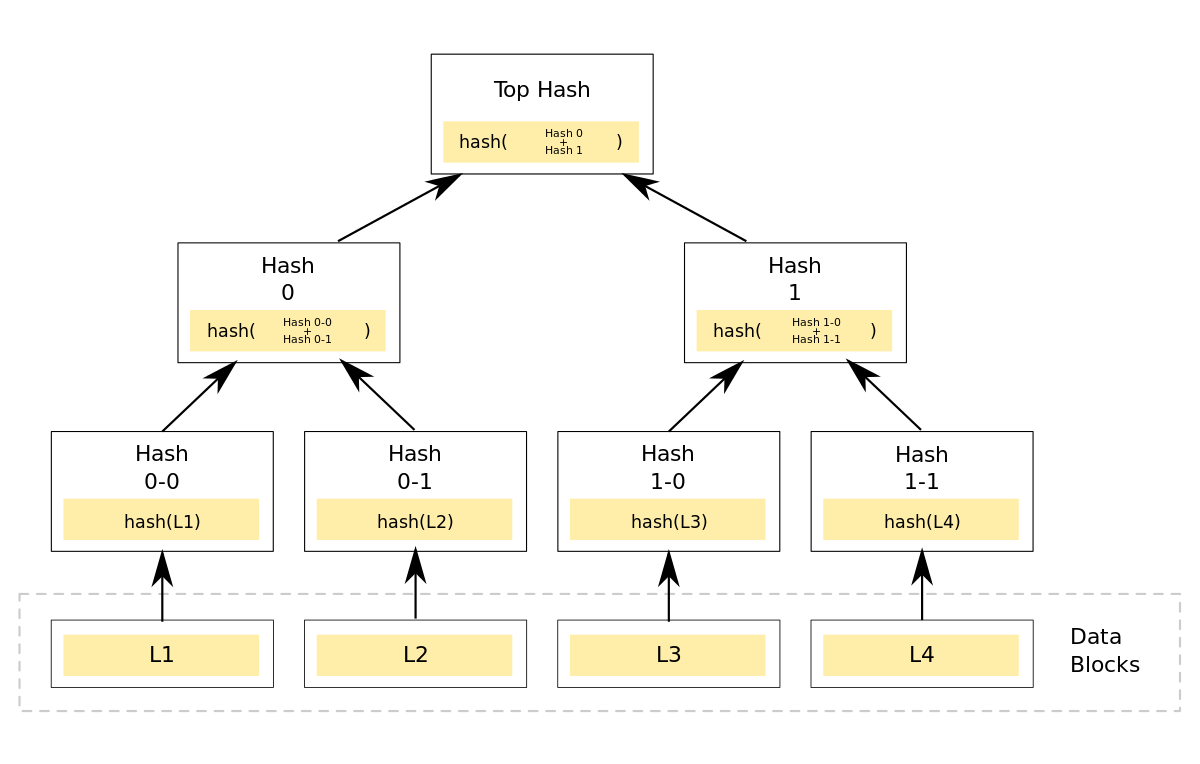
\includegraphics[width=1\columnwidth]{merkleTree}
	\captionsource{Merkle tree construction}{Merkle tree construction}
	{\url{https://en.wikipedia.org/wiki/Merkle_tree}}
	\label{fig:merkleTree}
\end{figure}

Given the top hash or the Merkle root and a leaf, it is possible to prove the
membership by giving the path for each complementary hashes. E.g given the
Merkle root and \texttt{L1}, the proof is \texttt{Hash 0-1} and \texttt{Hash 1}.
The verifier can then compute the hash of \texttt{L1}, the result of this hash
with \texttt{Hash 0-1}, and then with \texttt{Hash 1}. If the result is the same
as the Merkle root, then \texttt{L1} is a part of the tree.

In a block, the miner creates a Merkle tree of all included transaction
identifiers and puts the Merkle root into the header of the block. To validate
if a transaction is included in a block the path must be provided. Then the
resulting hash is compared to the Merkle root registered in the block's header.

% -----------------------------------------------------------------------------
\section{Transactions}

Transactions allow users to move Bitcoins from an address to another and they
create the content of the Bitcoin's blockchain. In Bitcoin, the blockchain does
not store a balance for each user; the blockchain keeps only the history of all
transactions made since the beginning.

\subsection{A list of inputs \& outputs}

A transaction is composed of a list of inputs and a list of outputs. In other
words, where the Bitcoins come from and where they go. Input refers to an
address where the funds will be spent, and output refers to an address where the
funds will go. An input points to another transaction output which has not been
used already. Inputs and outputs are links, to spend funds the user needs to
control addresses where unspent outputs are present. These unspent outputs are
called \texttt{UTXOs} and represent the total amount own by a user.

\begin{figure}[H]
	\centering
	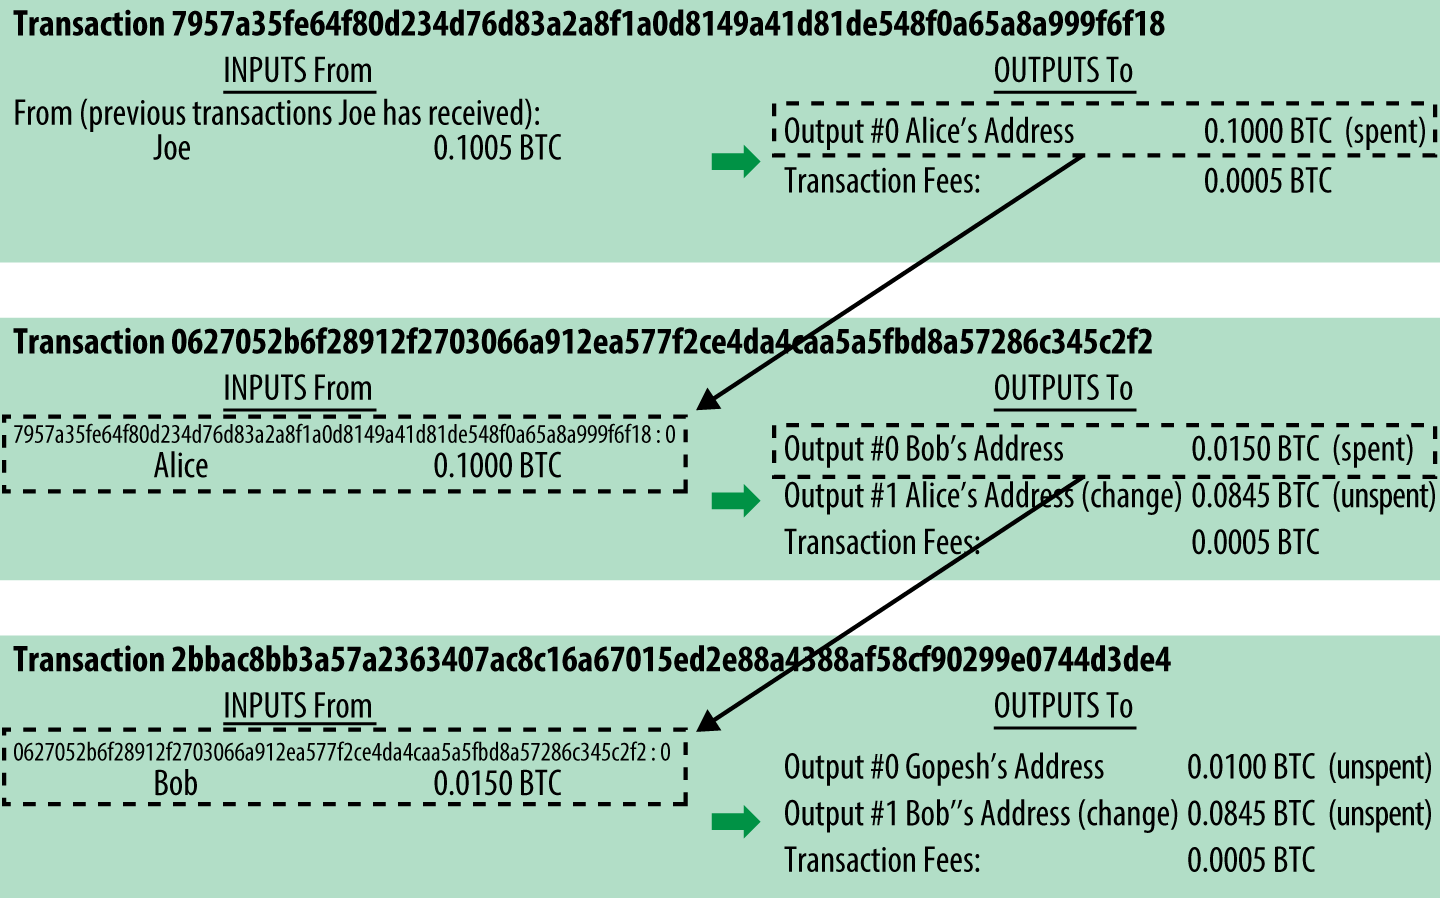
\includegraphics[width=1\columnwidth]{utxosChain}
	\captionsource{A chain of transactions where inputs and outputs are linked}
  {A chain of transactions where inputs and outputs are linked}
	{\url{https://github.com/bitcoinbook/bitcoinbook/blob/second_edition/ch02.asciidoc}}
	\label{fig:utxosChain}
\end{figure}

Each input is attached to a value (the value specified in the output to which
the input points). The sum of all inputs in a transaction must correspond to the
sum of all the values specified in the outputs, as in a dual entry accounting.
So an input must be spent entirely.

So, the most straightforward transaction is composed of one input and one output
with the same amount of money in and out. However, the most typical transaction
is composed of one input, referring to where the funds come from, and two
outputs. Indeed, it is scarce to have the right amount available in one
\texttt{UTXO}. So, the first output is the user who will receive the funds, with
the amount transferred, and the second output is another address owned by the
sender to gather the change, i.e., the remaining amount.

As blocks, transactions have an identifier. These identifiers are created in the
same way as blocks, by taking the double hash of the data, i.e., the signed
transaction. That means that, in the original design, a transaction does not
have its final transaction identifier (TXID) before she is wholly signed (every
input).

\subsection{Transaction fees}

The sum of all inputs in a transaction must correspond to the sum of all the
values specified in the outputs, yes but if the sum of all outputs is lower than
the sum of the inputs, the difference is implicitly considered as a fee (as
shown in Figure~\ref{fig:utxosChain}.) No fee was required in the beginning, but
today a transaction will not be included in a block without paying fees. A
miner, when he finds a block, can create the first transaction without inputs,
where a fixed amount of new coins is created plus the total amount of fees
collected in all the included transactions. A miner will, therefore, select the
transactions that pay the more fees concerning the amount of work needed to
validate them. Fees are calculated with the size of the transaction in bytes,
and a ratio of fee per byte then selected to find the fee for a transaction.

\subsection{Scripting language}

As described before, outputs or \texttt{UTXOs}, are related to addresses and
proof of ownership is required to spend them. To achieve the spending the
Bitcoin protocol uses digital signatures. To spend a \texttt{UTXO}, a valid
signature for to the address, and so the public key is required and to sign a
transaction the private key is required. Thus, while signing a transaction
corresponding to the right address, it is possible to prove that the user owns
the address. However, the protocol does not just require signatures and public
keys, conditions to \textit{unlock} a \texttt{UTXO} are structured in scripts.
Bitcoin has a stack-based script language called \say{Bitcoin Script}.

\begin{figure}[H]
	\centering
	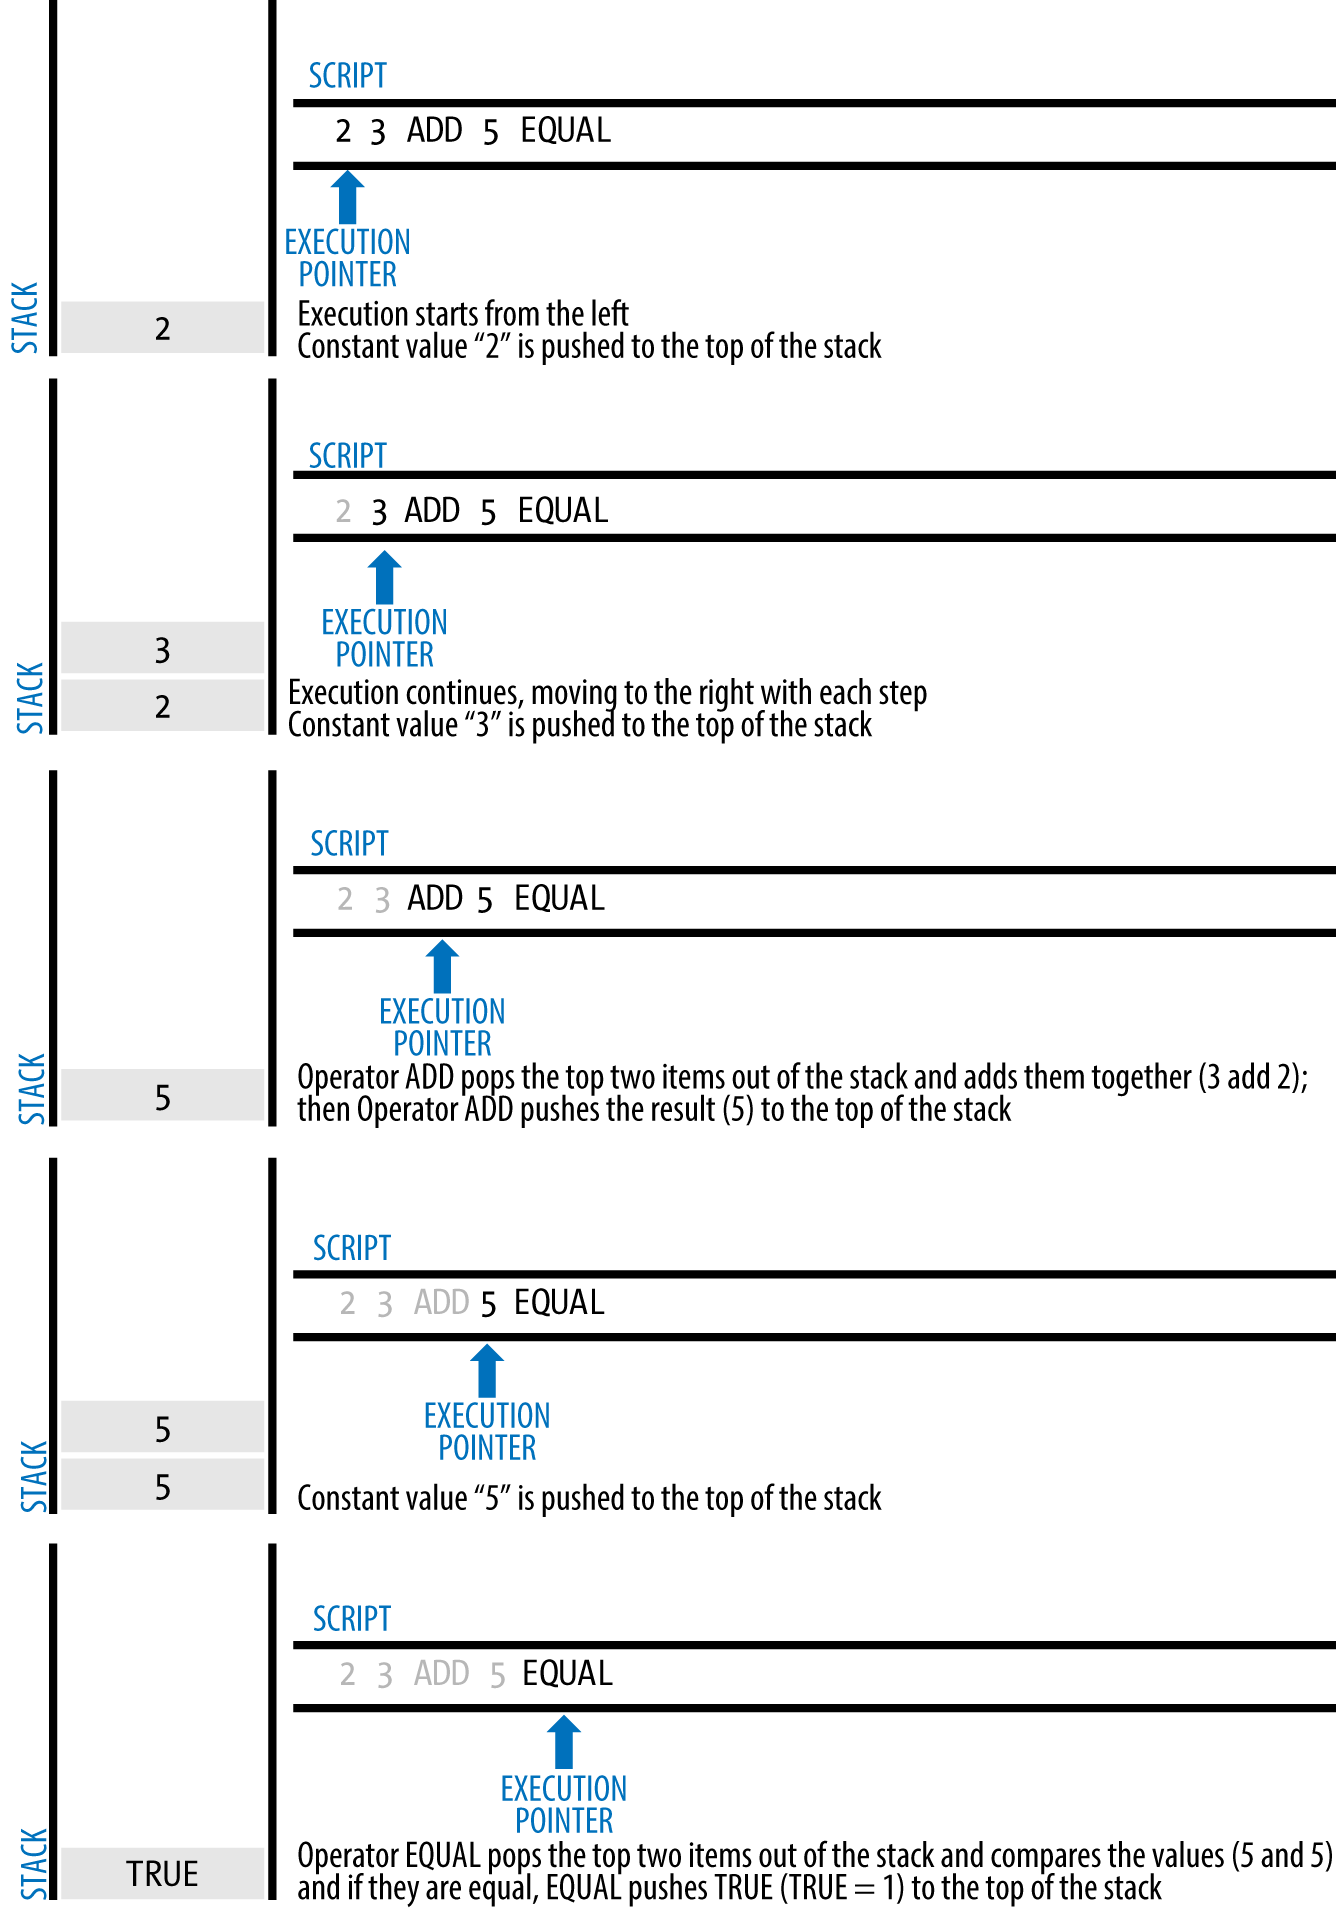
\includegraphics[width=0.73\columnwidth]{stackBased}
	\captionsource{Example of simple Bitcoin script program execution}
  {Example of simple Bitcoin script program execution}
	{\url{https://github.com/bitcoinbook/bitcoinbook/blob/second_edition/ch06.asciidoc}}
	\label{fig:stackBased}
\end{figure}

The list of all the \texttt{OP\_CODES} available in the Bitcoin script language
is in the documentation. Among them, \texttt{OP\_CHECKSIG} verify a given
signature with a public key provided onto the stack, \texttt{OP\_IF, OP\_ELSE,
OP\_ENDIF} create execution branch with a boolean onto the stack,
\texttt{OP\_DUP} duplicates the value onto the stack or \texttt{OP\_HASH160,
OP\_SHA256} compute hashes of values onto the stack.

Each input and output have a script. For output, the script corresponds to the
requirement to be fulfilled to be allowed to spend it. An address is the result
of the public key hashed with a \texttt{SHA256} and then hashed with a
\texttt{RIPEMD160} encoded with a checksum in a more human-readable format. A
user can decode the human-readable format of an address to retrieve the hash
data and create an output script called \gls{p2pkh}. With the script, the
address is retrieved, and given the address and the script, only the user who
holds the private key corresponding will be able to sign the transaction and
spend the funds. The user owning the address can create a transaction such as
input points to the \texttt{UTXO}. To unlock the funds, the user needs to sign
the transaction and give the signature with the public key in the input's
unlocking script. Before including a transaction in a candidate block, a miner
validates all the inputs. He needs to check if the pointed output is a
\texttt{UTXO}, so if the pointed output is \textit{unspent}, and execute the
locking script with the unlocking script. Both scripts are concatenated to
validate input; the unlocking script first (as shown in
Figure~\ref{fig:lockUnlock}).

\begin{figure}[H]
	\centering
	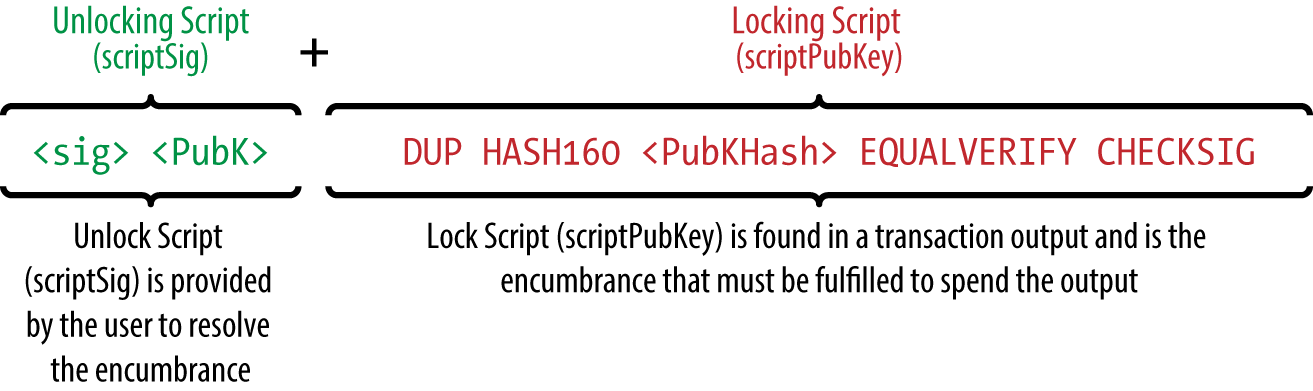
\includegraphics[width=1\columnwidth]{lockUnlock}
	\captionsource{Example of pay to public key hash script}
  {Example of pay to public key hash script}
	{\url{https://github.com/bitcoinbook/bitcoinbook/blob/second_edition/ch06.asciidoc}}
	\label{fig:lockUnlock}
\end{figure}

The script in Figure~\ref{fig:lockUnlock}, when executed, put the signature on
top of the stack, then the public key. The public key is duplicated, and hashed,
the public key hash present in the locking script is put on top of the stack,
and the two first element on top of the stack are then compared. If the
comparison failed, the script would fail and the transaction is rejected. If the
test pass, the signature will be checked with the two remaining parameters onto
the stack: the public key and the signature. If the signature is valid, the
value \texttt{True} is put on top of the stack. Otherwise, the script put the
value \texttt{False} on top of the stack. If the value \texttt{True} is present
on top of the stack at the end of the script the transaction is valid,
otherwise, the transaction is invalid.

\subsection{Segregated witness}

\gls{segwit} is the \gls{bip} 141 that propose to change the transaction
structure to fix transaction malleability, add script versioning, and improve
other aspects \cite{SegWit, SegWitBIP}. In fact, \gls{segwit} change the way
outputs are structured, the malleability is fixed if all inputs use \gls{segwit}
only. A transaction can have \gls{segwit} inputs and non-\gls{segwit} inputs at
the same time. The \gls{bip} abstract explains the purpose of \gls{segwit}:

\begin{quote}
  This BIP defines a new structure called a \say{witness} that is committed to
  blocks separately from the transaction merkle tree. This structure contains
  data required to check transaction validity but not required to determine
  transaction effects. In particular, scripts and signatures are moved into this
  new structure.

  The witness is committed in a tree that is nested into the block's existing
  merkle root via the coinbase transaction for the purpose of making this BIP
  soft fork compatible. A future hard fork can place this tree in its own branch.
\end{quote}

With \gls{segwit}, a transaction has two TXID. The first is determine without
all the witness data, so it is deterministic at the transaction creation. The
second one is related to the witness data and change when signatures appear.
This separation fixes the transaction malleability. The second big change is the
way the size is calculated to determine the fees. The transaction weight
\texttt{Tx Weight} becomes $\texttt{Base Tx} * 3 + \texttt{Total Size}$ where
\texttt{BaseTx} is the size without the witness data and \texttt{Total Size} is
the serialized transaction with all the data, including the witness data. With
this new structure the fees calculation change. The new structure introduce a
virtual transaction size such as virtual size is equal to $\texttt{Tx Weight} /
4$. Thus, \gls{segwit} reduce the weight of the witness data in the calculus of
the fees.

\subsection{Transaction malleability}

The fact that transaction identifier depends on the hash of the serialized
transaction while the signature does not currently cover all the data in a
transaction introduce what is called transaction malleability. Indeed, a miner
can tweak the transaction to change is identifier before including it into a
block without invalidating it nor changing the claiming output conditions. This
malleability means that an unconfirmed chain of transactions must not be trusted
(because the following transactions will depend on the hashes of the previous
transactions.)

The first way to achieve malleability is to tweak the signatures themselves. For
every signature $(r, s)$, the signature $(r, -s \pmod n)$ is a valid signature
for the same message. As mentioned in the Bitcoin wiki about transaction
malleability:

\begin{quote}
	As of block 363724, the BIP66 soft fork has made it mandatory for all new
	transactions in the block chain to strictly follow the DER-encoded ASN.1 standard.
	Further efforts are still under way to close other possible malleability within
	DER signatures.
\end{quote}

However, even if the format is standardized and enforced, signatures can still
be changed by anyone who has access to the corresponding private keys. When the
user signs a transaction, the unlocking script (scriptSig) contains, e.g., for a
standard \gls{p2pkh}, the signature and the public key. These data are present
in the signed transaction, but cannot be present during the signing process
because they do not yet exist. This presence of signatures in the script means
that the content of unlocking scripts are not part of the signing data, but part
of the hashing data for the TXID. E.g., by introducing an additional
\texttt{OP\_CODE}, it is possible to change the TXID without invalidating the
signature.

Nevertheless, with \gls{segwit} activated, now the transaction malleability with
signatures and scripts is no longer possible. As mentioned in the \gls{bip}:

\begin{quote}
	It allows creation of unconfirmed transaction dependency chains without
	counterparty risk, an important feature for offchain protocols such as the
	Lightning Network.
\end{quote}


% -----------------------------------------------------------------------------
\section{Scalability of Bitcoin}

Improvements on the consensus layer have been made and will continue to appear
to answer the problem of scalability. However, modifying the consensus layer is
not easy, usually soft forks are needed, and the process can be painful. With
\gls{segwit}, the latest significant improvement on-chain, all the prerequisites
to construct a robust layer-two application, such as fixing malleability, are
fulfilled.

\subsection{Layer-two applications}

The layer-two is an architectural concept where a blockchain is used as a source
of truth and only for resolving disagreements. Usually, the construction that
uses this architectural concept is called payment channels or micropayment
channels. These channels enable scalability because they reduce the number of
transactions needed on the blockchain if two users often exchange.
